\begin{appendices}
	\crefalias{chapter}{appcha}
	\crefalias{section}{appsec}
	\renewcommand{\thesection}{\Alph{chapter}\arabic{section}}

	\chapter{Additional results from \cref{cha:obesity_genetic_signatures_and_cancer}}
	\label{app:a}

	\section{Metagenes created from raw data vs. standardised data (Creighton)}
	\label{sec:metagenes_created_from_raw_data_vs_standardised_data}
	
	\begin{figure}[htpb]
		\centering
		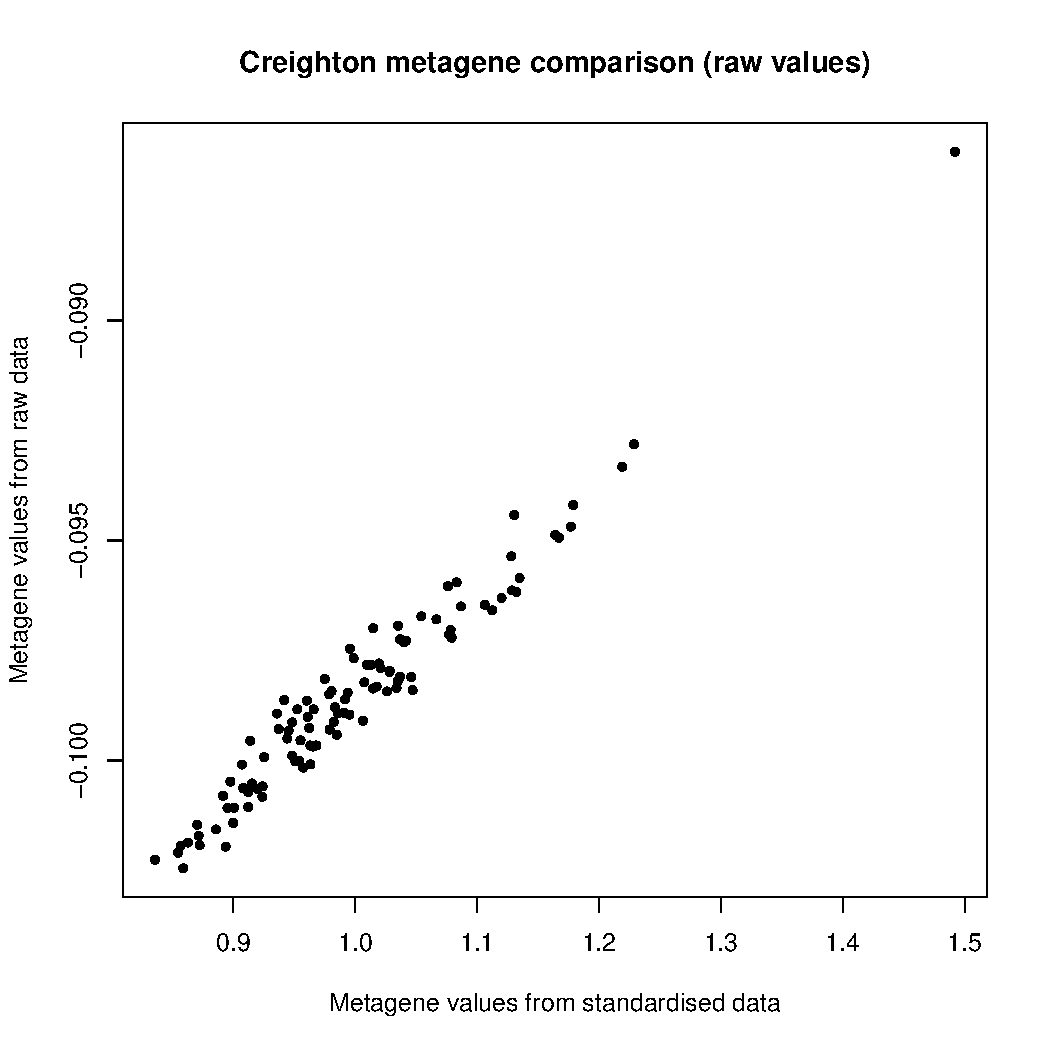
\includegraphics[width=0.45\linewidth,page=1]{appendix/check_raw_vs_std_mg}
		\hfill
		\includegraphics[width=0.45\linewidth,page=2]{appendix/check_raw_vs_std_mg}
		\caption{appendix/Check_raw_vs_std}
		\label{fig:appendix/check_raw_vs_std}
	\end{figure}
	
	\section{Metagenes created from raw data vs. standardised data (ICGC)}
	\label{sec:metagenes_created_from_raw_data_vs_standardised_data_icgc}

	\begin{figure}[htpb]
		\centering
		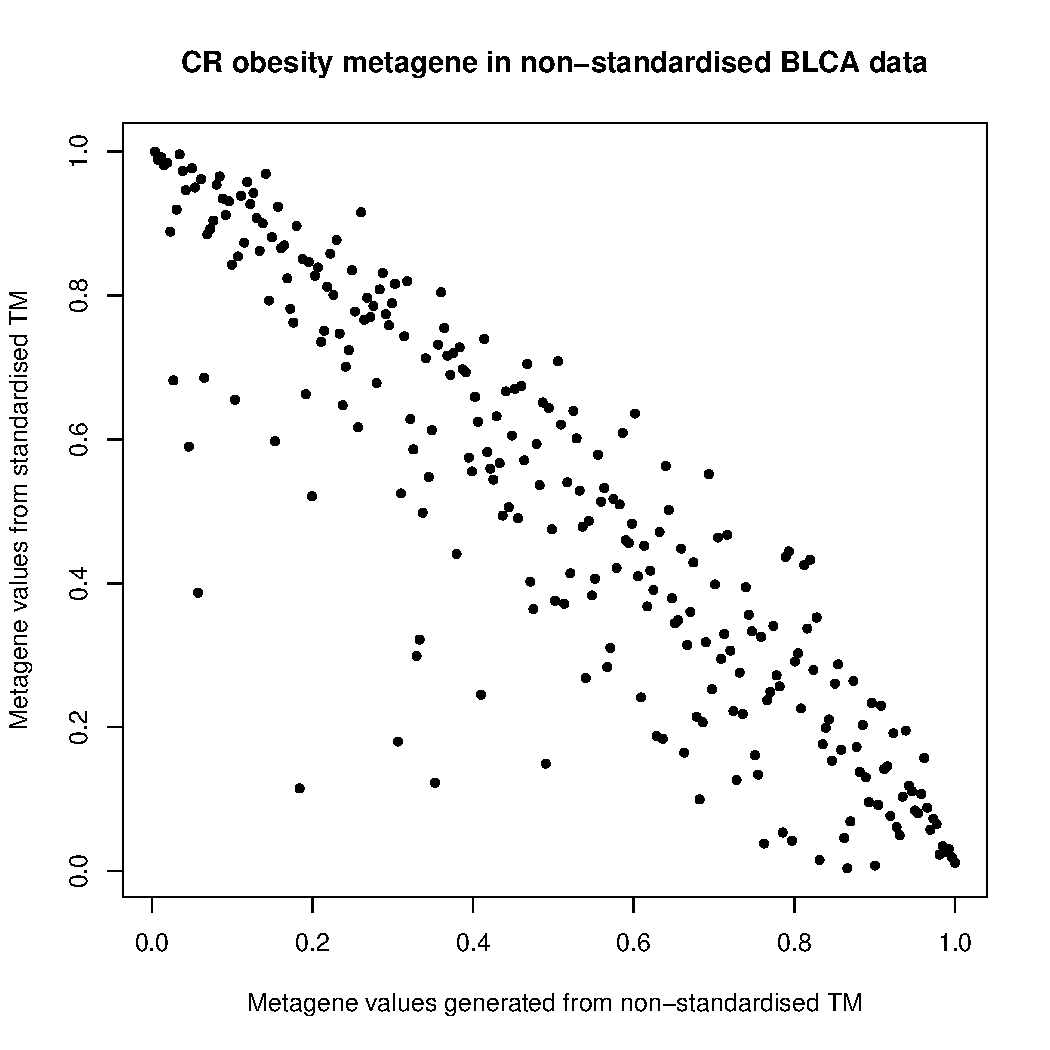
\includegraphics[width=0.45\linewidth,page=1]{appendix/crtcga_raw_vs_std}
		\hfill
		\includegraphics[width=0.45\linewidth,page=2]{appendix/crtcga_raw_vs_std}
		\caption{appendix/Check_raw_vs_std}
		\label{fig:appendix/check_raw_vs_std}
	\end{figure}

	\section{Rest of the ICGC cancer heatmap resutls}
	\label{sec:rest_of_the_icgc_cancer_heatmap_resutls}
	
	\begin{figure}[htpb]
		\centering
		\includegraphics[width=0.45\linewidth,page=1]{appendix/crtcga_std}
		\hfill
		\includegraphics[width=0.45\linewidth,page=2]{appendix/crtcga_std}
		\caption{appendix/Check_raw_vs_std}
		\label{fig:appendix/check_raw_vs_std}
	\end{figure}

	\section{FM metagene, raw vs std}
	\label{sec:fm_metagene_raw_vs_std}
	
	\begin{figure}[htpb]
		\centering
		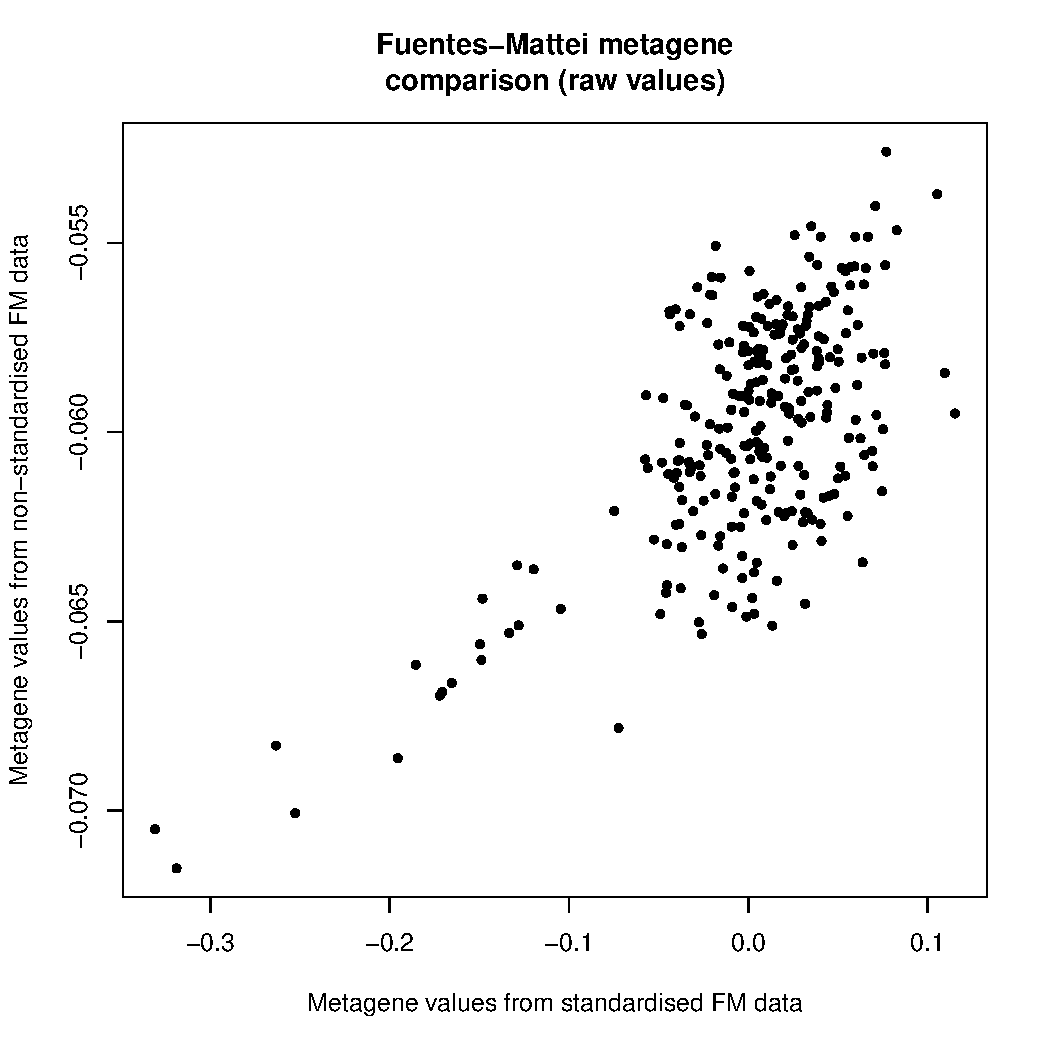
\includegraphics[page=1,width=0.8\linewidth]{appendix/fm_meta_check}
		\caption{appendix/fm_meta_check}
		\label{fig:appendix/fm_meta_check}
	\end{figure}
	

	\section{Creighton DEG metagene direction}
	\label{sec:creighton_deg_metagene_direction}
	
	\begin{figure}[htpb]
		\centering
		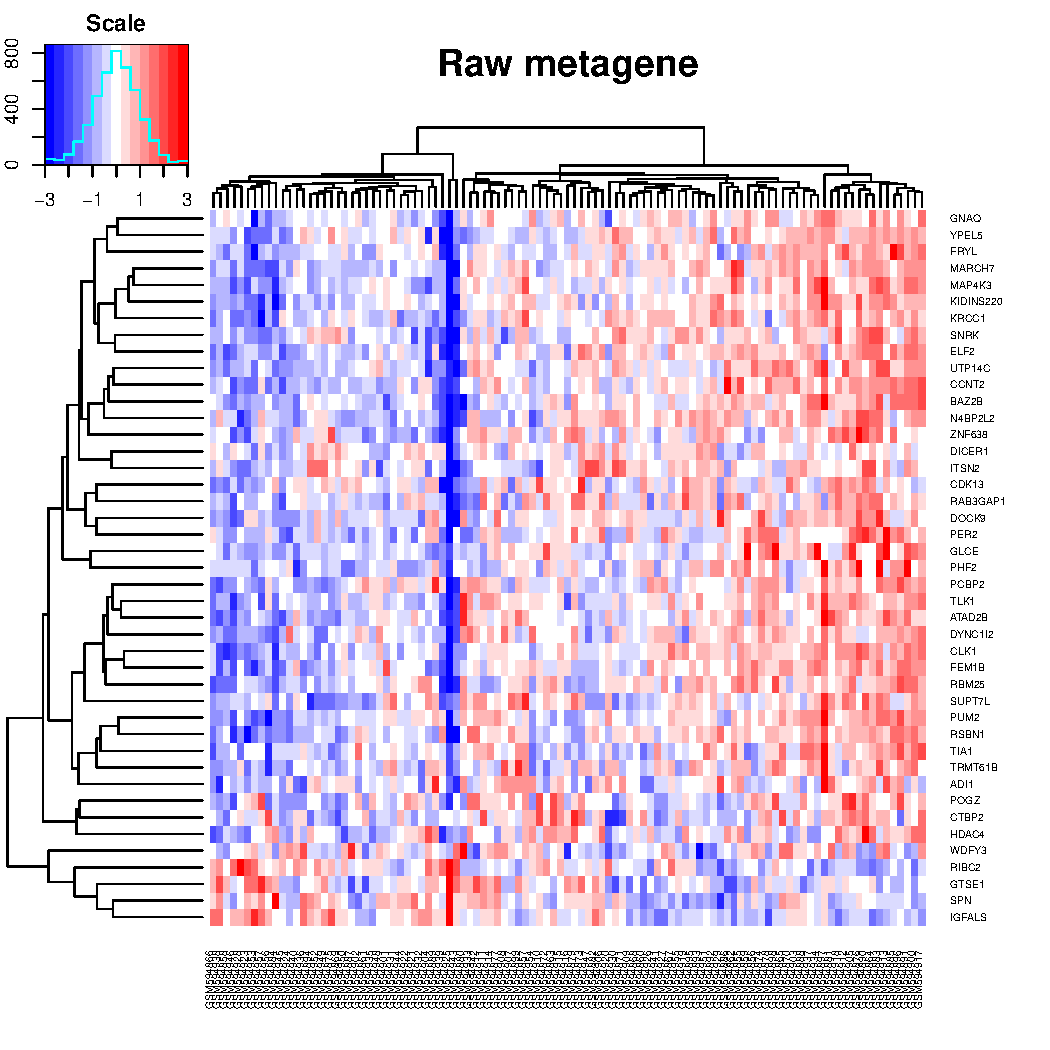
\includegraphics[page=1,width=0.8\linewidth]{cr_meta_direction}
		\caption{cr_meta_direction}
		\label{fig:cr_meta_direction}
	\end{figure}
	
	
	\section{Number of gene probes/genes in each signature}
	\label{app:number_of_gene_probes_genes_in_each_signature}
	
	\begin{table}[htbp]
		\centering
		\caption{Summary of the number of gene probes and genes in each obesity associated genetic signature}
		\label{tab:signature_gene_num}
		\begin{tabular}{lcc}
			Obesity associated genetic signature & No. gene probes   & No. genes\\
			\hline
			\rule{0pt}{2.25ex}Original & 799 & 644\\
			Cr                         & 799 & 678\\
			Res                        & 799 & 655\\
			Ca                         & 799 & 657\\
			CaRes                      & 799 & 651\\
			CrOl                       & 239 & 199\\
			ResOl                      & 168 & 147\\
			CaOl                       & 148 & 128\\
			CaResOl                    & 92  & 86\\
			\hline
			\hline
		\end{tabular}
	\end{table}

	\chapter{Additional results from \cref{cha:obesity_associated_genetic_signature_and_pathway_signatures}}
	\label{app:b}

	\begin{figure}[htpb]
		\centering
		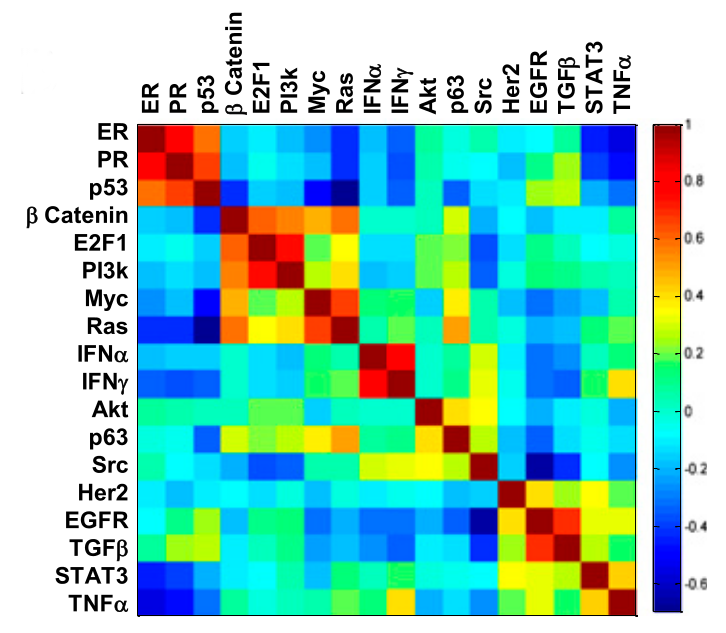
\includegraphics[width=0.7\linewidth]{results2/gatzares1}
		\caption{results from gatza's study}
		\label{fig:gatza_paper_res}
	\end{figure}



\end{appendices}
